\documentclass[xcolor=dvipsnames]{beamer}
\usepackage{graphicx,url}
\renewcommand{\S}[0]{\mathrm{S}}
\renewcommand{\P}[0]{\mathrm{P}}
% example themes
%\usetheme{Frankfurt}
%\usecolortheme{seahorse}
%\usecolortheme{rose}

\newcommand{\st}{\, | \,}

\renewcommand{\arraystretch}{1.2}

% put page numbers
% \setbeamertemplate{footline}[frame number]{}
\setbeamertemplate{frametitle}[default][center]
% remove navigation symbols
\setbeamertemplate{navigation symbols}{}

\title{Seeded Inflation/Deflation Ranking}
\institute{HLTCOE Mini-SCALE}
\author{Vince Lyzinski \\ Pushpendre Rastogi \\ Jeremy Silver}
\begin{document}

\frame[plain]{\titlepage}

\begin{frame}{The Inflation Ranking Method}
  \vspace{7pt}
  \begin{table}[htbp]
    \centering
    \begin{tabular}{l|l}
      \textbf{Given} & A set of points $\{p_i \st i \in [1, \ldots, \mathrm{P}]\}$ \\
            & A set of seeds $\{s_j \st j \in [1, \ldots, \mathrm{S}]\}$   \\
      \end{tabular}
  \end{table}

  \pause
  \vspace{-10pt}
\begin{table}[htbp]
  \centering
  \begin{tabular}{|r|l|}%\toprule
    \multicolumn{2}{ c }{\textit{Some Definitions}}\\\hline
    $d_{ij}$ &  Distance of point $p_i \in \mathbb{R}^d$ from seed $s_j \in \mathbb{R}^d$\\
    $\ell_j$ & Signed, weighted label of $s_j$\\
    $c_{i}(r) = \underset{j \st d_{ij} \le r}{\sum} \ell_j$ & Sum of labels of seeds
                 within distance $r$\\\hline
    \end{tabular}
  \end{table}
\pause
  \textbf{The Inflation Ranking Rule}:  $p_{i} > p_{i'}$ if there exists $r_0$ such that
  $c_{i}(r_0) > c_{i'}(r_0)$, and $c_{i}(r) = c_{i'}(r)$ for all $r < r_0$.
\pause
  \begin{table}[htbp]
    \centering
    \begin{tabular}{|r|l|}
      \multicolumn{2}{c}{\textit{Properties}}\\\hline
      Strict Weak Ordering & Proved \\
      Efficient & $O(\S\P\log(\S\P))$ \\
      Evaluation & \textit{See below} \\\hline
      \end{tabular}
  \end{table}

\end{frame}

\begin{frame}{Inflation Ranking: Example}
\begin{figure}
  \makebox[\textwidth][c]{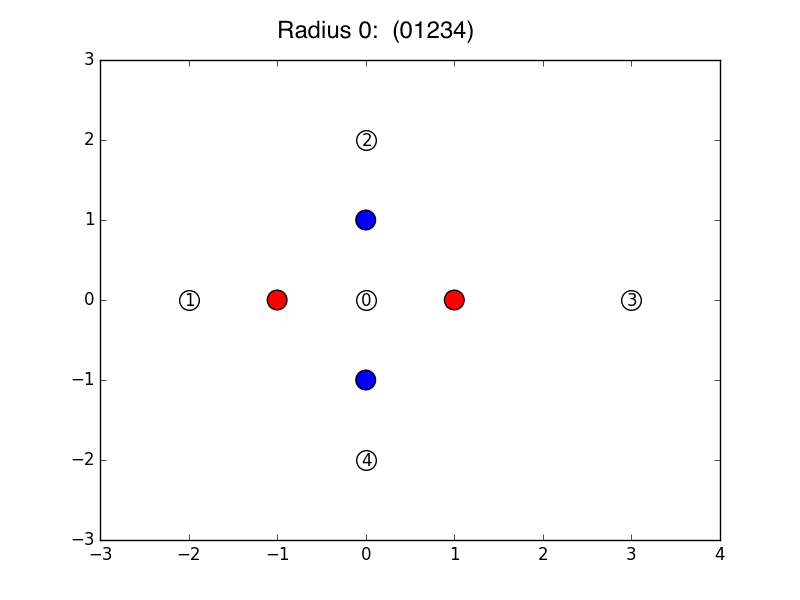
\includegraphics[width=1.05\textwidth]{img/tie_r0.png}}
\end{figure}
\end{frame}

\begin{frame}{Inflation Ranking: Example}
\begin{figure}
  \makebox[\textwidth][c]{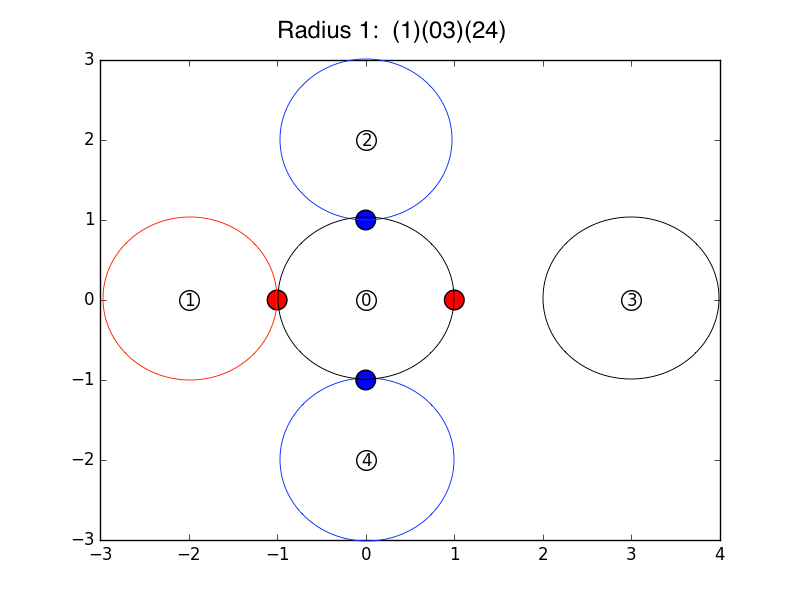
\includegraphics[width=1.05\textwidth]{img/tie_r1.png}}
\end{figure}
\end{frame}

\begin{frame}{Inflation Ranking: Example}
\begin{figure}
  \makebox[\textwidth][c]{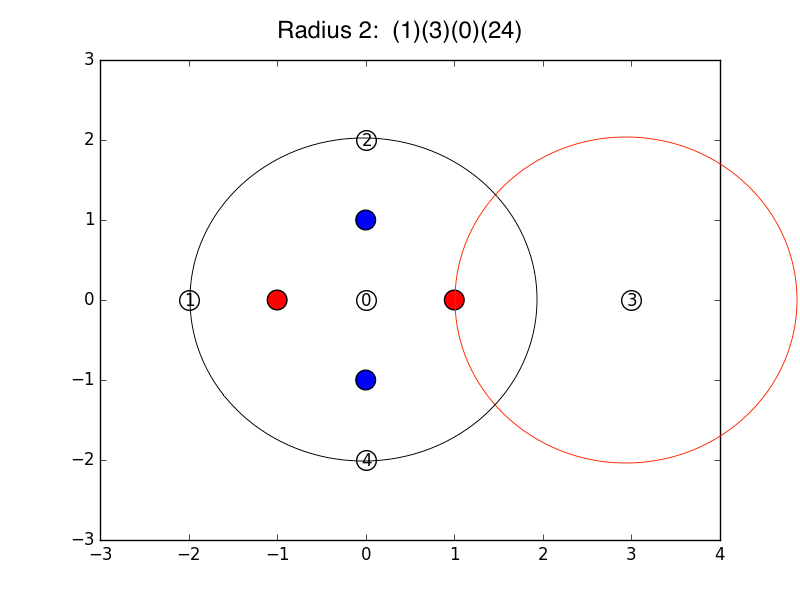
\includegraphics[width=1.05\textwidth]{img/tie_r2.png}}
\end{figure}
\end{frame}
\begin{frame}
\textbf{The Inflation Ranking Rule}:  $p_{i} > p_{i'}$ if there exists $r_0$ such that
$c_{i}(r_0) > c_{i'}(r_0)$, and $c_{i}(r) = c_{i'}(r)$ for all {\color{red}$r \mathbf{<} r_0$}

\vspace{5em}

\textbf{The Deflation Ranking Rule}:  $p_{i} > p_{i'}$ if there exists $r_0$ such that
  $c_{i}(r_0) > c_{i'}(r_0)$, and $c_{i}(r) = c_{i'}(r)$ for all {\color{red}$r \mathbf{>} r_0$}
\end{frame}


\begin{frame}{Inflation \& Deflation Ranking in $\mathbb{R}^2$}
\begin{figure}
  \makebox[\textwidth][c]{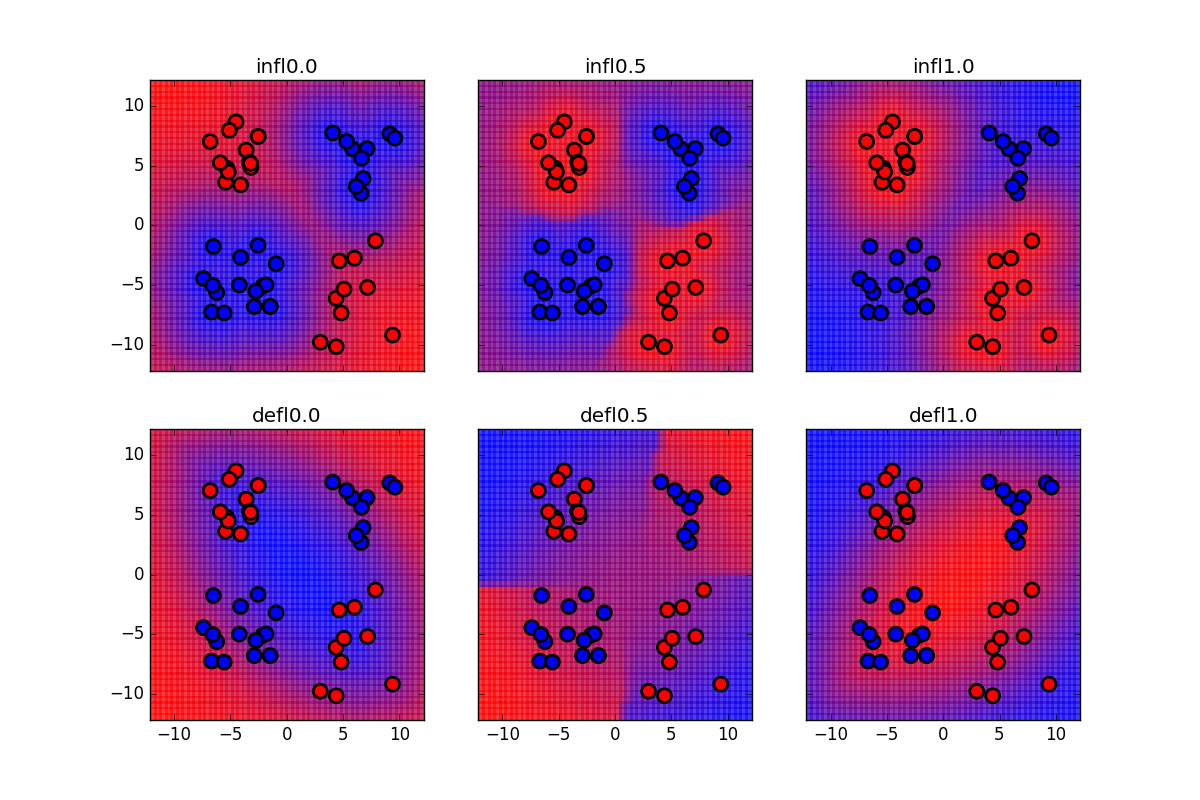
\includegraphics[width=1.2\textwidth]{img/square1_balloon.png}}
\end{figure}
\end{frame}


\begin{frame}{Inflation \& Deflation Ranking in $\mathbb{R}^2$}
\begin{figure}
  \makebox[\textwidth][c]{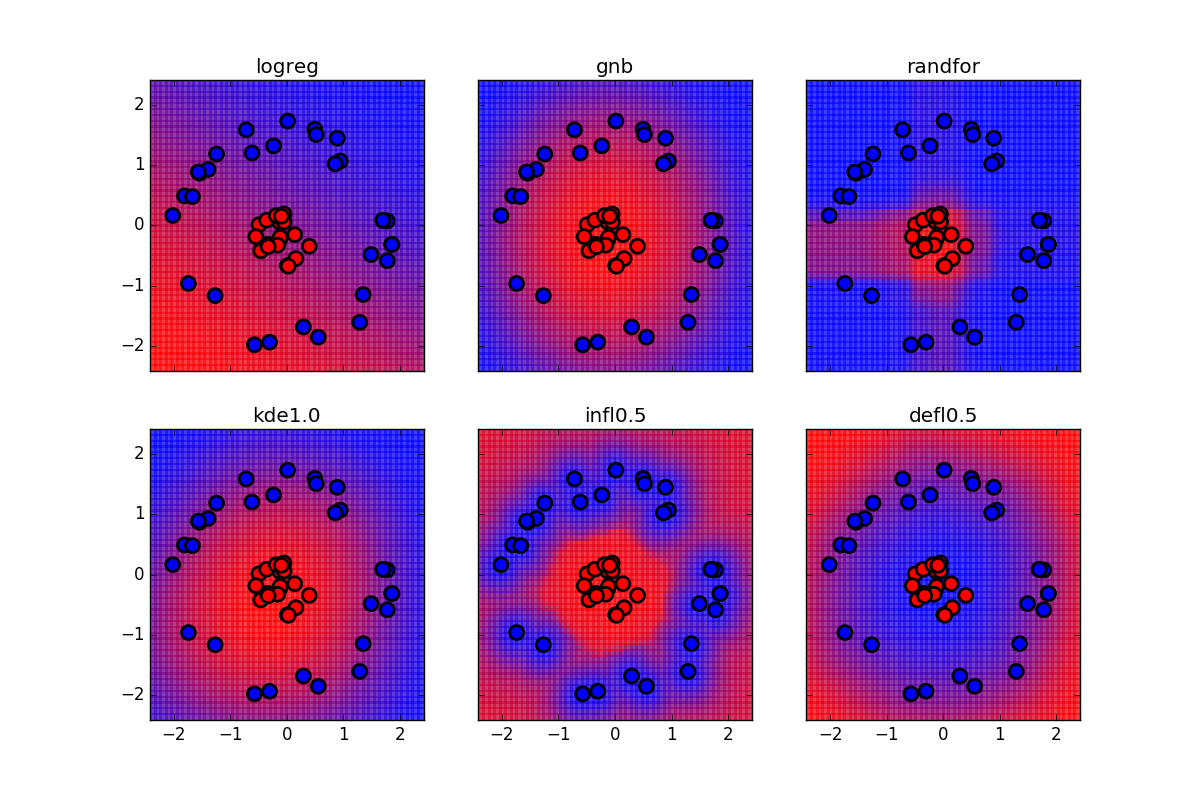
\includegraphics[width=1.2\textwidth]{img/target_compare.png}}
\end{figure}
\end{frame}

\begin{frame}{Inflation \& Deflation Ranking in $\mathbb{R}^2$}
\begin{figure}
  \makebox[\textwidth][c]{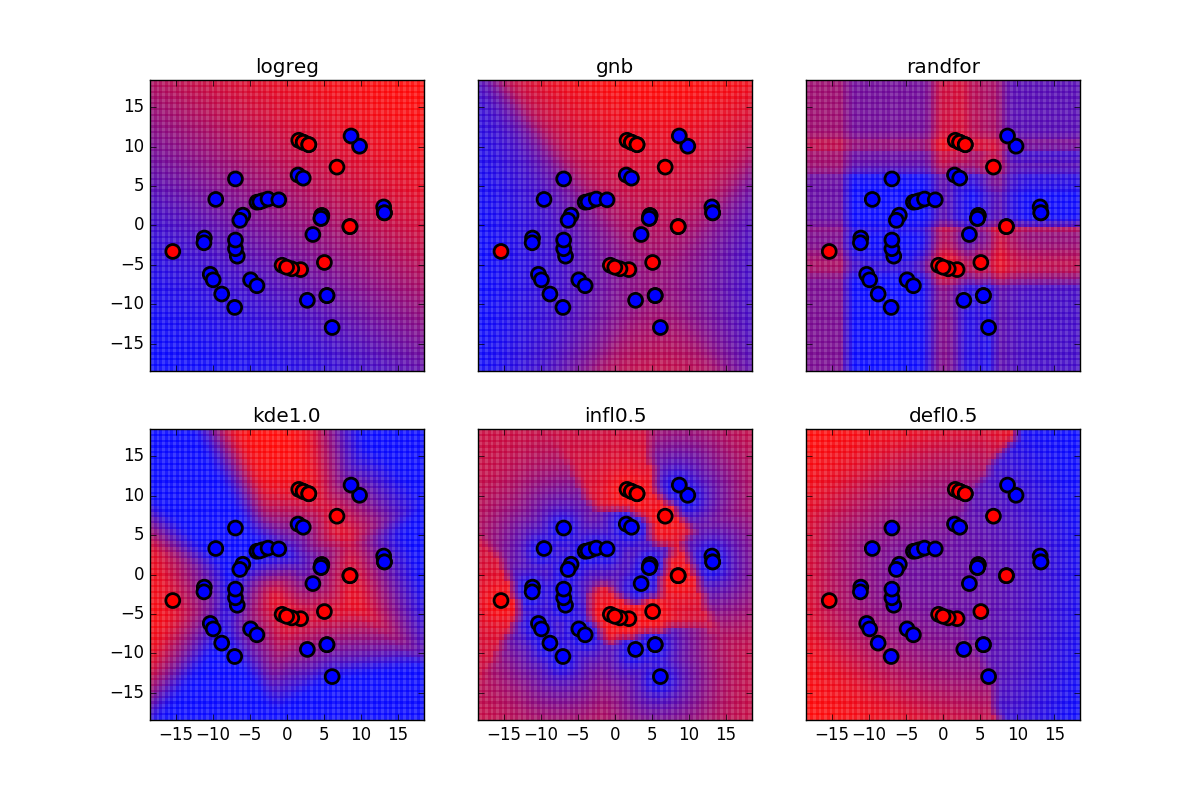
\includegraphics[width=1.2\textwidth]{img/3-spiral_compare.png}}
\end{figure}
\end{frame}

\begin{frame}{Vertex Nomination Evaluation (Google+)}
\begin{figure}
  \makebox[\textwidth][c]{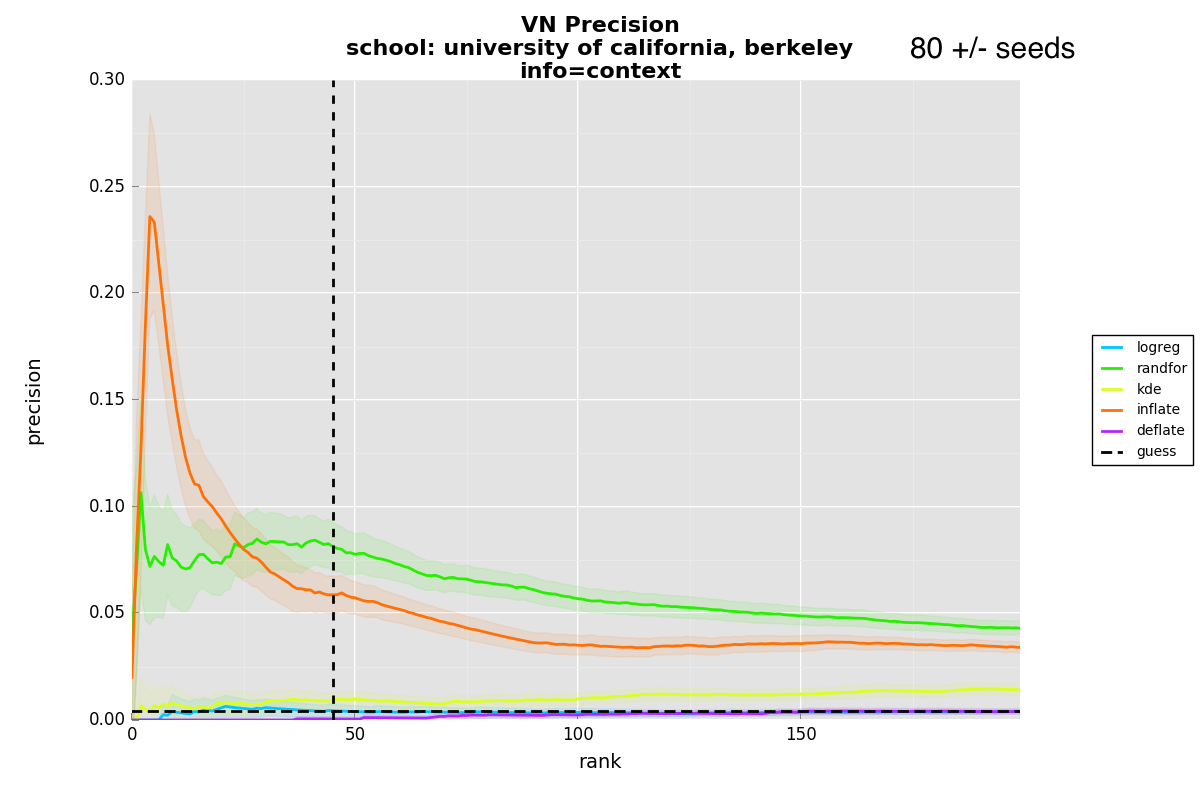
\includegraphics[width=1.1\textwidth]{img/uc_berkeley.png}}
\end{figure}
\end{frame}

\begin{frame}{Vertex Nomination Evaluation (Google+)}
\begin{figure}
  \makebox[\textwidth][c]{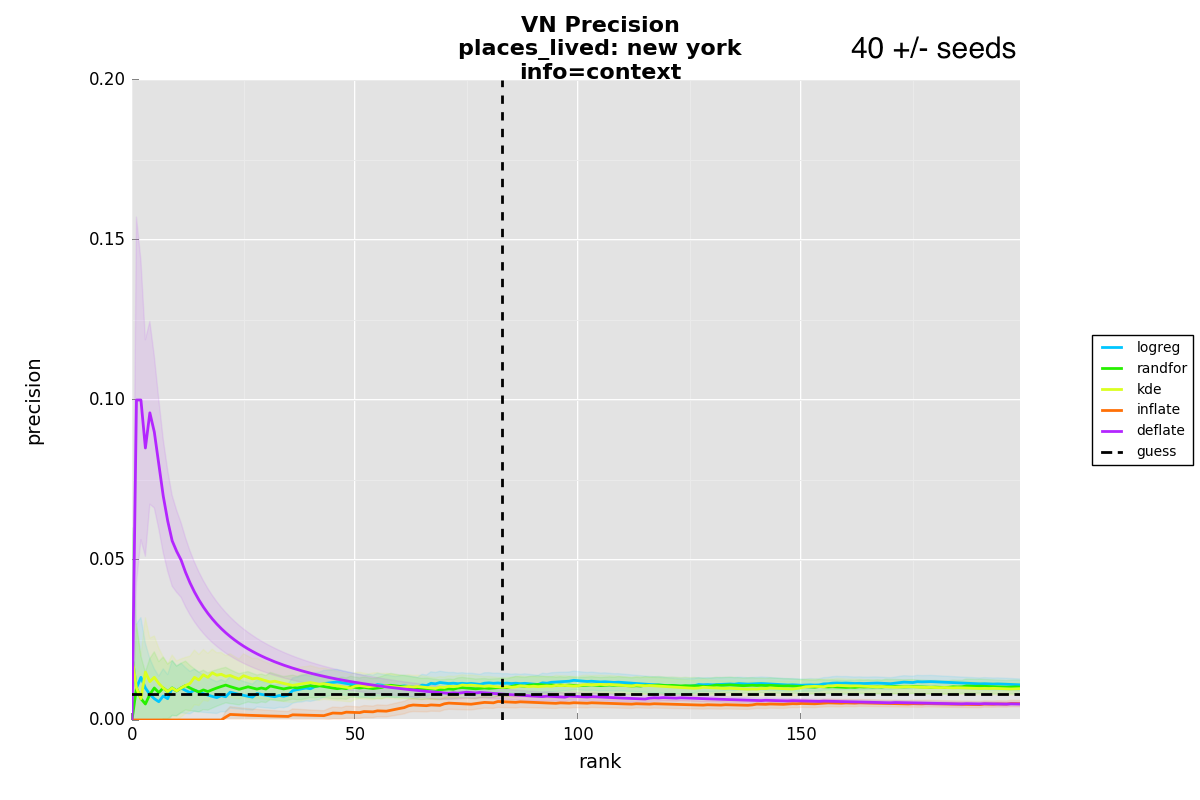
\includegraphics[width=1.1\textwidth]{img/new_york.png}}
\end{figure}
\end{frame}

\end{document}


%%% Local Variables:
%%% mode: latex
%%% TeX-master: t
%%% End:
